\section{General Statistics}
To get a broad overview of the dataset we decided to make some general numerical analysis of the dataset to get a feeling for Spotify playlists as data and the scope of the dataset. In the dataset there are \var{SizeDataset} playlists\footnote{Originally there are 1 million playlists. Due to limited processing power we had to reduce our analysis to a dataset of \var{SizeDataset} playlists.} with a total number of \var{unique_tracks} unique tracks by \var{artists_unique} artists in \var{albums_unique} albums. The total length of all playlist is \var{converted_total_duration}.

The average number of tracks in one playlist are $\approx$ \var{approx_average_numtracks}\footnote{The exact number are \var{average_numtracks} tracks} tracks. Figure \ref{fig:averagetrack} shows how the average number of tracks per playlists changes, when more and more playlists are considered. 

\begin{figure}[ht]
    \centering
    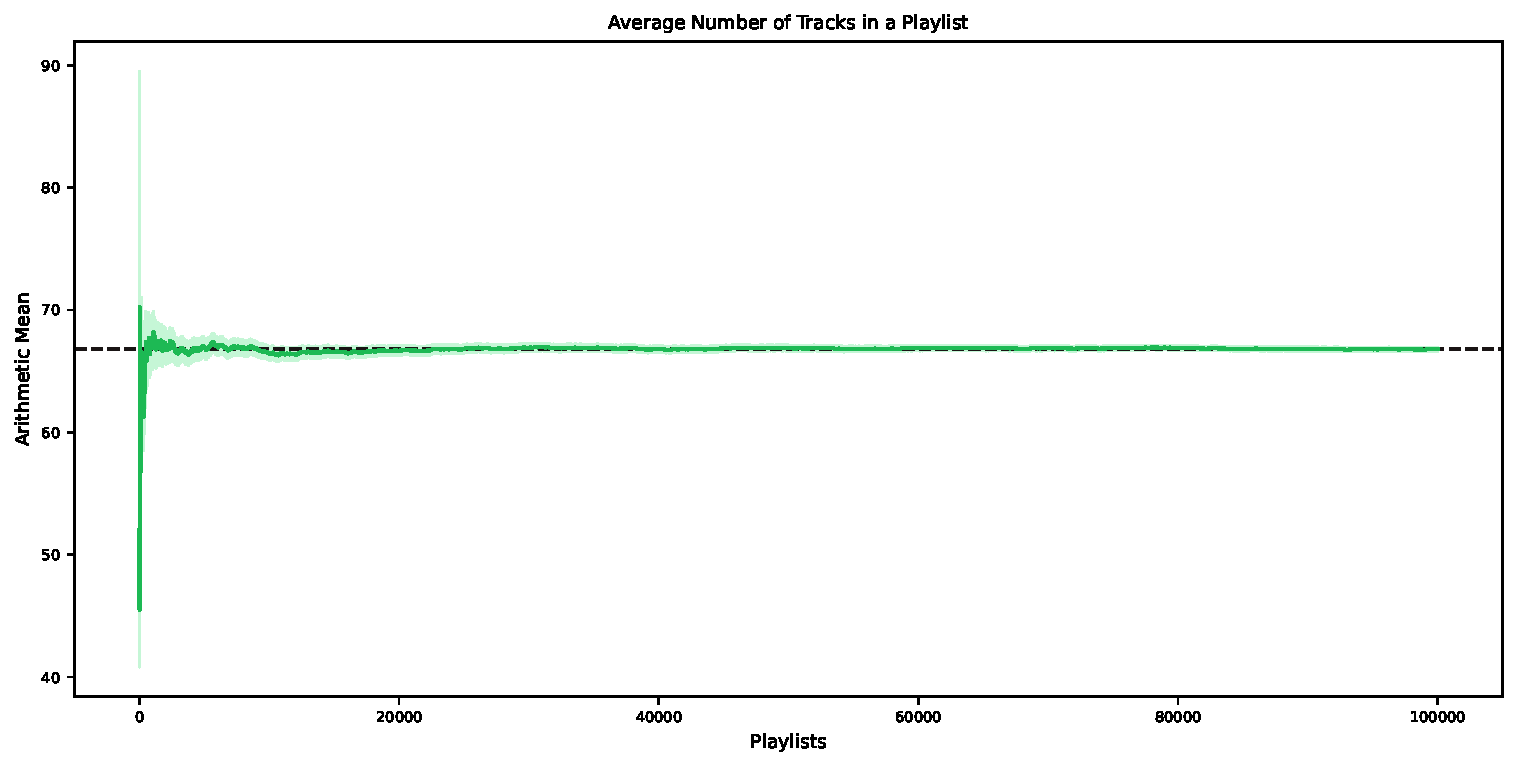
\includegraphics[width=\textwidth]{fig/averageTrack.pdf}
    \caption{CAPTION}
    \label{fig:averagetrack}
\end{figure}

The average duration of a playlist is \var{converted_average_duration}. This fits (approximately) with the fact, that a track has an average duration of \var{converted_average_track_duration}.\footnote{Using the following calculation:\\$\text{average duration of track [ms]}\cdot\text{average number of tracks in a playlist}=\var{average_track_duration} \text{ ms}\cdot\var{average_numtracks}= \var{cal_average_playlist_duration} \text{ ms} = $ \var{converted_cal_average_playlist_duration}}

\begin{figure}[ht]
    \centering
    \includegraphics[width=0.3\textwidth]{fig/CumUniqueness.png}
    \includegraphics[width=0.3\textwidth]{fig/CumUniqueness.png}
    \includegraphics[width=0.3\textwidth]{fig/CumUniqueness.png}
    \label{fig:cumUniqueness}
\end{figure}

\answerTODO{} TEXT for cumsum graphs

To get the most popular tracks, albums and artists, we counted how often they were occurring in a playlist. The result ca be seen in figure \ref{fig:popular}. The top 15 tracks are expectedly matching with the first 15 billboard charts of 2017 \cite{BillboardMedia}.

\begin{figure}[ht]
    \centering
    \includegraphics[width=0.3\textwidth]{fig/TopTracks.png}
    \includegraphics[width=0.3\textwidth]{fig/TopAlbums.png}
    \includegraphics[width=0.3\textwidth]{fig/TopPopularArtits.png}
    \caption{CAPTION}
    \label{fig:popular}
\end{figure}